\documentclass{standalone}
\usepackage{tikz}
\usepackage{pgfplots}
\pgfplotsset{compat=1.18}
\usetikzlibrary{intersections}

\begin{document}
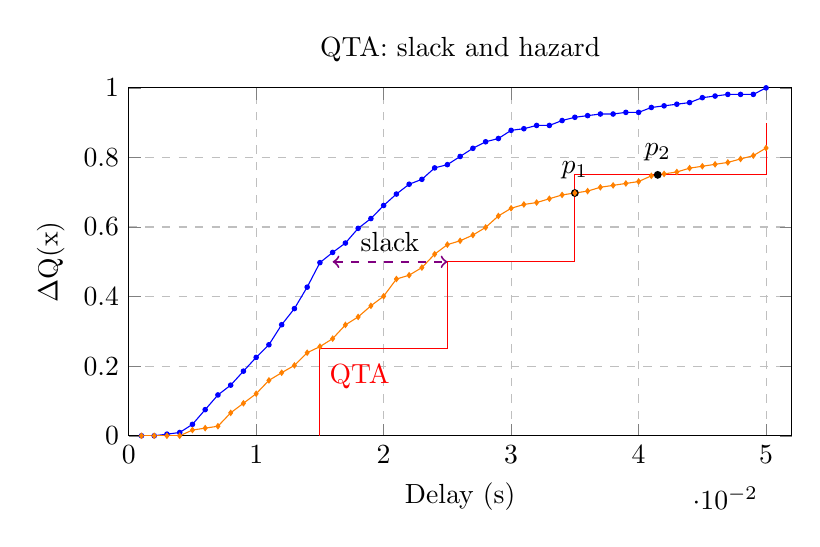
\begin{tikzpicture}[ dot/.style = {circle, fill, semitransparent, inner sep=2pt}]
\begin{axis}[
        title={QTA: slack and hazard},
    xlabel={Delay (s)},
    ylabel={$\Delta$Q(x)},
    xmin=0, xmax=0.052,
    ymin=0, ymax=1,
    xtick={0, 0.01, 0.02, 0.03, 0.04, 0.05},
    ytick={0,0.2,0.4,0.6,0.8,1},
    ymajorgrids=true,
    xmajorgrids=true,
    grid style=dashed,
    width=10cm,
    height=6cm,
]

% Main CDF plot
\addplot[color=blue, mark=*, mark size = 0.8pt] coordinates {
    (0.001, 0.000000)
    (0.002, 0.000000)
    (0.003, 0.004695)
    (0.004, 0.009390)
    (0.005, 0.032864)
    (0.006, 0.075117)
    (0.007, 0.117371)
    (0.008, 0.145540)
    (0.009, 0.185709)
    (0.010, 0.225352)
    (0.011, 0.261690)
    (0.012, 0.319249)
    (0.013, 0.365587)
    (0.014, 0.427230)
    (0.015, 0.497653)
    (0.016, 0.527042)
    (0.017, 0.553991)
    (0.018, 0.596244)
    (0.019, 0.624413)
    (0.020, 0.661972)
    (0.021, 0.694836)
    (0.022, 0.723005)
    (0.023, 0.737089)
    (0.024, 0.769953)
    (0.025, 0.779343)
    (0.026, 0.802817)
    (0.027, 0.826291)
    (0.028, 0.845070)
    (0.029, 0.854460)
    (0.030, 0.877934)
    (0.031, 0.882629)
    (0.032, 0.892019)
    (0.033, 0.892019)
    (0.034, 0.906103)
    (0.035, 0.915493)
    (0.036, 0.920188)
    (0.037, 0.924883)
    (0.038, 0.924883)
    (0.039, 0.929577)
    (0.040, 0.929577)
    (0.041, 0.943662)
    (0.042, 0.948357)
    (0.043, 0.953052)
    (0.044, 0.957746)
    (0.045, 0.971831)
    (0.046, 0.976526)
    (0.047, 0.981221)
    (0.048, 0.981221)
    (0.049, 0.981221)
    (0.050, 1.000000)
};

\addplot[color=orange, mark=diamond*, mark size = 0.9pt, name path=A1] coordinates {
    (0.001, 0.000000)
    (0.002, 0.000000)
    (0.003, 0.000000)
    (0.004, 0.000000)
    (0.005, 0.016484)
    (0.006, 0.021978)
    (0.007, 0.027473)
    (0.008, 0.065934)
    (0.009, 0.093407)
    (0.010, 0.120879)
    (0.011, 0.159341)
    (0.012, 0.181319)
    (0.013, 0.202308)
    (0.014, 0.238791)
    (0.015, 0.256264)
    (0.016, 0.279231)
    (0.017, 0.318681)
    (0.018, 0.341648)
    (0.019, 0.373626)
    (0.020, 0.401099)
    (0.021, 0.450549)
    (0.022, 0.461538)
    (0.023, 0.483516)
    (0.024, 0.521978)
    (0.025, 0.549451)
    (0.026, 0.560440)
    (0.027, 0.576923)
    (0.028, 0.598901)
    (0.029, 0.631868)
    (0.030, 0.653846)
    (0.031, 0.664835)
    (0.032, 0.670330)
    (0.033, 0.681319)
    (0.034, 0.692308)
    (0.035, 0.697802)
    (0.036, 0.703297)
    (0.037, 0.714286)
    (0.038, 0.719780)
    (0.039, 0.725275)
    (0.040, 0.730769)
    (0.041, 0.747253)
    (0.042, 0.752747)
    (0.043, 0.758242)
    (0.044, 0.769231)
    (0.045, 0.774725)
    (0.046, 0.780220)
    (0.047, 0.785714)
    (0.048, 0.795714)
    (0.049, 0.805198)
    (0.050, 0.827143)
};

\addplot[color=red, mark=none, name path = A2] coordinates {
    (0.015, 0)
    (0.015, 0.25)
    (0.025, 0.25)
    (0.025, 0.5)
    (0.035, 0.5)
    (0.035, 0.75)
    (0.05, 0.75)
    (0.05, 0.9)
}
node[pos=0.25,below right] {QTA}
;

\draw[line width = 0.25mm,color=violet, dashed, <->, label=slack] (0.016, 0.5) -- (0.025,0.5) node[pos=0.5, above, black] {slack};


\path[name intersections={of=A1 and A2,name=i,total=\t}]
     foreach \X in {1,2}{(i-\X) node[black,circle,fill,inner sep=1pt, label=$p_\X$]{}};

\end{axis}
\end{tikzpicture}
\end{document}
